% --------------------------------- Overfitting, Underfitting, and Model Optimization ---------------

\section{Overfitting, Underfitting, and Model Optimization}
\label{sc:overfitting}
In the previous examples—temperature forecasting, classifying drought severity, and modeling lake water temperatures—we observed a common trend: the performance of the model on held-out validation data often peaked after a few training epochs and then began to degrade. This phenomenon, where a model performs well on training data but poorly on unseen data, is known as \textit{overfitting}. Overfitting is a challenge faced in every deep learning project, and mastering strategies to combat it is crucial for building effective models.
At the heart of this challenge is the tension between \textbf{optimization} and \textbf{generalization}:
Optimization refers to the process of training a model to perform as well as possible on the training data. Essentially, this is the \textit{learning} in DL. Generalization, on the other hand, is the ability of the trained model to perform well on unseen data.
Our ultimate goal is to achieve good generalization. However, generalization cannot be directly controlled during training; we can only adjust the model based on its performance on the training data. Understanding this balance is key to building robust models for hydrology and environmental sciences.
At the beginning of training, optimization and generalization are typically aligned: as the model's performance on the training data improves, so does its performance on validation data. During this stage, the model is said to be \textit{underfitting}. Underfitting occurs when the model has not yet captured all the relevant patterns in the training data, leaving room for improvement.

However, after a certain number of training iterations, a turning point is reached where the performance on the validation data stops improving. Beyond this point, continued optimization on the training data causes the model to overfit. \textit{Overfitting occurs when the model begins to memorize patterns that are specific to the training data} rather than learning generalizable patterns. These irrelevant patterns do not translate well to unseen data, leading to degraded performance on the validation set.

The most effective way to prevent overfitting is to \textit{increase the amount of training data}. With more diverse and representative data, the model can naturally generalize better to unseen examples. However, in many cases—especially in hydrology and environmental sciences—collecting additional data can be costly, time-consuming, or even impossible due to physical and logistical constraints.
When more data is not an option, the next-best approach is to restrict the amount of information the model can store or impose constraints on how it learns. This ensures the model focuses on the most relevant patterns in the data, which are more likely to generalize well. Techniques that achieve this are collectively referred to as \textbf{regularization}, which are discussed in section \ref{sc:reg}.


Regularization introduces constraints that limit a model's capacity to memorize irrelevant patterns, helping it generalize better. The underlying idea is simple: if a model can only "afford" to store a limited number of patterns, it will prioritize learning the most prominent and meaningful ones. Regularization methods include:


In the next section, we will explore these regularization techniques in detail and demonstrate how to apply them to improve the performance of a precipitation classification model.







\subsection{Weight Regularization}
\subsection{Early Stopping}
Early stopping is another effective technique for avoiding overfitting. It monitors the model’s performance on a validation set during training and stops training when performance on the validation set stops improving. This prevents the model from continuing to train and overfit the training data.

For example, a DL model might overfit after 100 epochs even though validation performance peaked at 50 epochs (\ref{fig:earlystop}). Early stopping stops the training process automatically, saving time and ensuring the best-performing model is retained.
In Keras, early stopping is implemented using the \textit{EarlyStopping} callback. For example:

\begin{lstlisting}[language=Python]
from keras.callbacks import EarlyStopping

# Define an EarlyStopping callback
early_stopping = EarlyStopping(monitor='val_loss', patience=5, restore_best_weights=True)

# Train the model 
model.fit(X_train, y_train, validation_data=(X_val, y_val), epochs=100, callbacks=[early_stopping])

\end{lstlisting}
Here:
\begin{itemize}
    \item \texttt{monitor= 'val\_loss'} tracks the validation loss.
    \item patience=5 means training stops if validation loss does not improve for 5 consecutive epochs.
    \item \texttt{restore\_best\_weights=True} ensures the best model is saved.
\end{itemize}

\subsection{Dropout Regularization}
Dropout is a simple yet powerful technique where a fraction of neurons in a layer is randomly "dropped out" during each training step. These dropped-out neurons do not contribute to the forward pass or the backward pass (gradient updates). This forces the network to learn more robust features by ensuring that no single neuron or group of neurons becomes overly specialized or reliant on specific connections.

For example, imagine a network that predicts runoff based on rainfall, temperature, and soil moisture. If some neurons are randomly deactivated during training, the network must learn alternative pathways and redundant features, improving its ability to generalize.

Key points about dropout:

\begin{itemize}
    \item Dropout is applied only during training, not during testing.
    \item The dropout rate specifies the fraction of neurons to drop (typically between 0.2 and 0.5).
    \item It works like training an ensemble of smaller subnetworks, which combine into a stronger overall model.
\end{itemize}
Adding dropout to a model in Keras is straightforward. For example:
\begin{lstlisting}[language=Python]
from keras.models import Sequential
from keras.layers import Dense, Dropout
# Define a model with dropout
model = Sequential([
    Dense(64, activation='relu', input_shape=(10,)),  # Input layer
    Dropout(0.3),  # Dropout layer with 30% rate
    Dense(32, activation='relu'),
    Dropout(0.2),  # Dropout layer with 20% rate
    Dense(1, activation='sigmoid')  # Output layer])
model.compile(optimizer='adam', loss='binary_crossentropy', metrics=['accuracy'])
\end{lstlisting}
\subsection{Batch Normalization}
\subsection{K-fold Cross-Validation}
K-fold cross-validation is a practical technique to evaluate model performance and reduce overfitting (discussed in detail in section \ref{sc:overfitting}), especially when data is limited. It works by dividing the dataset into k equal parts, called folds. For instance, if \textit{k=4}, the data is split into 4 subsets (Figure \ref{fig:kfold}). The model is trained on 3 folds and validated on the 1 remaining fold. This process is repeated 4 times, so each fold serves as the validation set exactly once. The final performance is averaged across all 4 runs, providing a robust estimate of the model's ability to generalize to new data.

This method ensures that all data points are used for both training and validation, making the most of limited datasets. For example, if the data is not shuffled before splitting, similar types of data (e.g., seasonal trends in hydrological data) might cluster in one fold, leading to biased results. By shuffling the data beforehand, each fold becomes more representative of the entire dataset, improving the reliability of the evaluation.

K-fold cross-validation is essential because it reduces the risk of overfitting. It ensures the model is tested on different subsets of data, exposing it to various patterns and reducing dependency on any single data split.



\begin{figure}[h!]
    \centering
    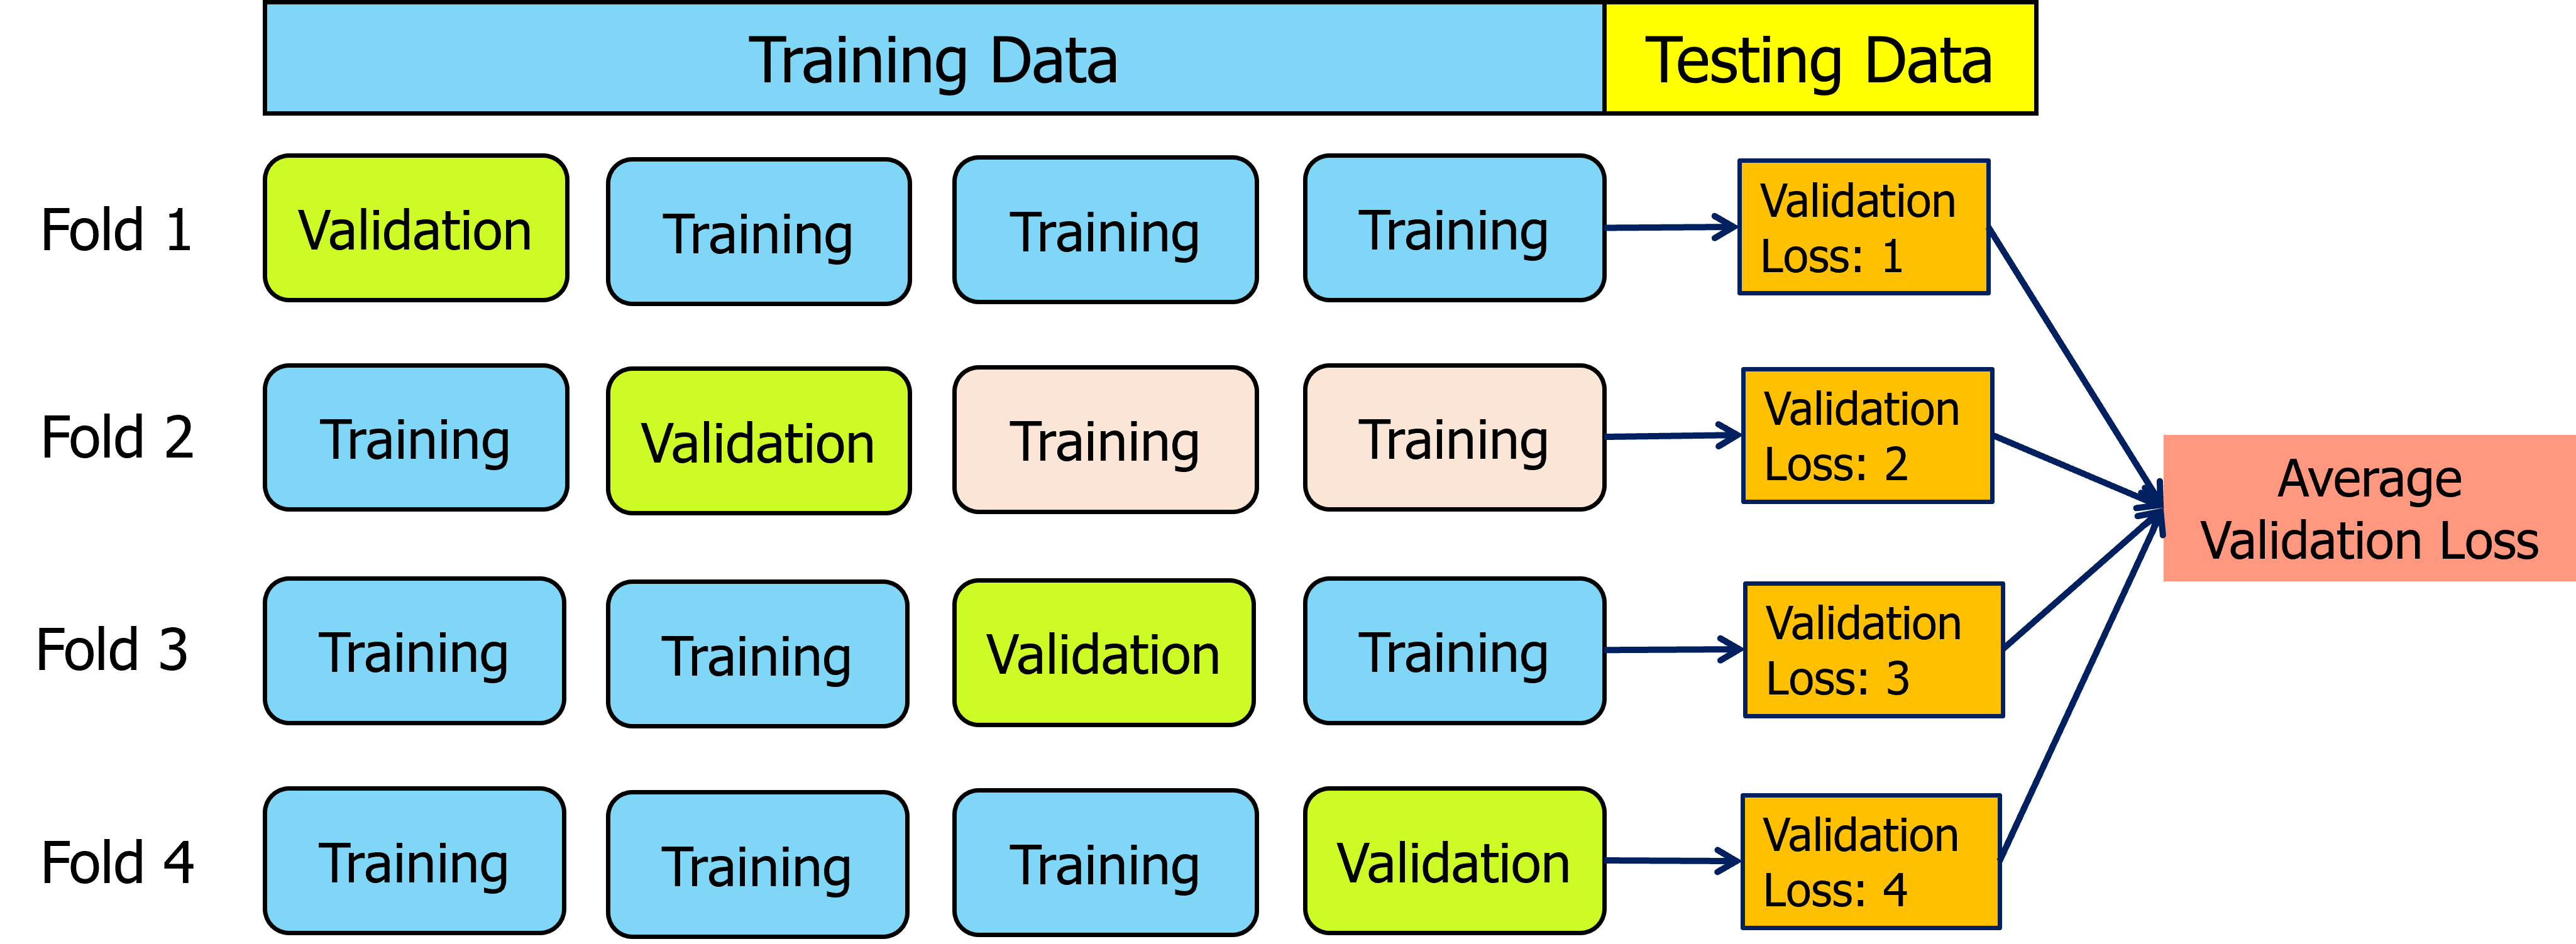
\includegraphics[width=\linewidth]{images/k-foldcrossval.png}
    \caption{K-fold Cross-Validation: The training data is divided into multiple subsets (folds). Each fold takes a turn as the validation set while the rest are used for training. The final validation score is the average of validation losses across all folds.}
    \label{fig:kfold}
\end{figure}


\begin{lstlisting}[language=Python]
# Example Python code for k-fold cross-validation with shuffling
from sklearn.model_selection import KFold
import numpy as np

data = np.array([...])  # Example data array
kfold = KFold(n_splits=5, shuffle=True, random_state=42)

for train, test in kfold.split(data):
    # Apply training and testing here
\end{lstlisting}